
% Figure 4: Non-Uniform Voltage Grid + ΔV-Weighted Metric
% Compile: pdflatex fig4_voltage_grid.tex
\documentclass[border=4pt]{standalone}
\usepackage{tikz}
\usepackage{amsmath,amssymb}
\usepackage{pgfplots}
\pgfplotsset{compat=1.18}
\usetikzlibrary{arrows.meta,calc,decorations.pathreplacing}

% ── ICML Global Colour System ──
\definecolor{ink}{HTML}{1F2937}
\definecolor{flagship}{HTML}{2563EB}
\definecolor{secondary}{HTML}{D97706}
\definecolor{physgood}{HTML}{059669}
\definecolor{errbad}{HTML}{BE123C}
\definecolor{muted}{HTML}{64748B}
\definecolor{panelbg}{HTML}{F8FAFC}
\definecolor{gridline}{HTML}{E2E8F0}
\definecolor{mppgold}{HTML}{F59E0B}

\begin{document}
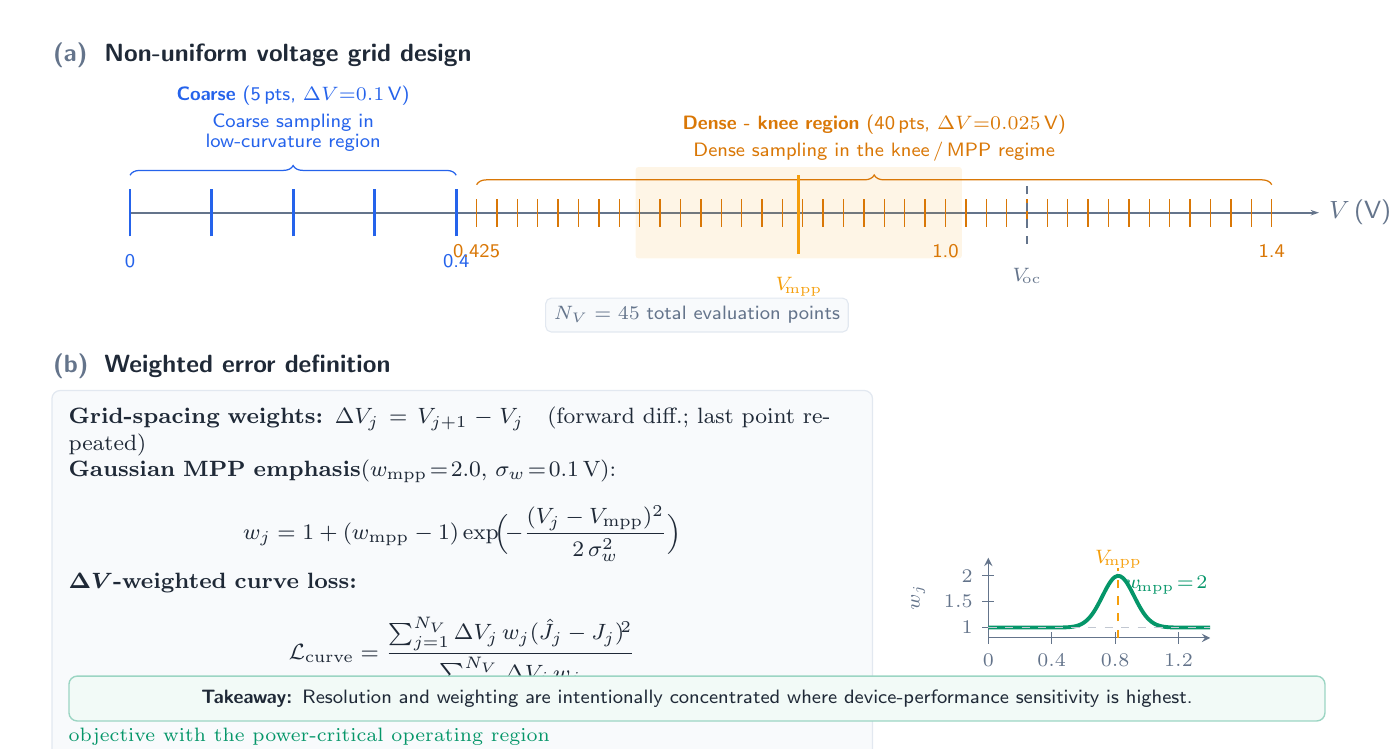
\begin{tikzpicture}[every node/.style={font=\sffamily,text=ink}]

% ── Canvas: 17.0 cm × 8.8 cm ──
\useasboundingbox (0,0) rectangle (17,8.8);

% ════════════════════════════════════════════════════
%  PANEL (a) - Non-uniform voltage grid design
% ════════════════════════════════════════════════════
\node[font=\sffamily\small\bfseries,text=muted,anchor=west]
  at (0.2,8.45) {(a)};
\node[font=\sffamily\small\bfseries,anchor=west]
  at (0.85,8.45) {Non-uniform voltage grid design};

% ── Axis geometry ──
\pgfmathsetmacro{\axL}{1.3}          % left end (cm)
\pgfmathsetmacro{\axR}{15.8}         % right end (cm)
\pgfmathsetmacro{\axY}{6.45}         % axis y-position
\pgfmathsetmacro{\vs}{(\axR-\axL)/1.4} % cm per volt

% Horizontal axis arrow
\draw[-{Stealth[length=3pt,width=2pt]},line width=0.7pt,muted]
  (\axL,\axY) -- (\axR+0.6,\axY)
  node[right,font=\sffamily\small,text=muted]{$V$\,(V)};

% ── MPP highlight zone (light alpha fill) ──
\fill[mppgold,opacity=0.10,rounded corners=1pt]
  ({\axL+0.62*\vs},{\axY-0.58})
  rectangle
  ({\axL+1.02*\vs},{\axY+0.58});

% ── Coarse ticks: 0-0.4 V, ΔV = 0.1 V, 5 points ──
\foreach \v in {0.0,0.1,0.2,0.3,0.4}{
  \pgfmathsetmacro{\xp}{\axL+\v*\vs}
  \draw[flagship,line width=1.0pt]
    (\xp,{\axY-0.30}) -- (\xp,{\axY+0.30});
}
% Endpoint labels
\node[below=3pt,font=\sffamily\scriptsize,text=flagship]
  at (\axL,{\axY-0.30}) {0};
\node[below=3pt,font=\sffamily\scriptsize,text=flagship]
  at ({\axL+0.4*\vs},{\axY-0.30}) {0.4};

% Coarse brace + annotation
\draw[decorate,
  decoration={brace,amplitude=3.5pt,raise=5pt},
  line width=0.45pt,flagship]
  (\axL,{\axY+0.30}) -- ({\axL+0.4*\vs},{\axY+0.30})
  node[midway,above=10pt,font=\sffamily\scriptsize,text=flagship,
       align=center,text width=4.2cm]{
    \textbf{Coarse} (5\,pts, $\Delta V{=}0.1$\,V)\\[1.5pt]
    Coarse sampling in\\[-0.5pt]low-curvature region
  };

% ── Dense ticks: 0.425-1.4 V, \DeltaV = 0.025 V, 40 points ──
\foreach \i in {0,1,...,39}{
  \pgfmathsetmacro{\v}{0.425+\i*0.025}
  \pgfmathsetmacro{\xp}{\axL+\v*\vs}
  \draw[secondary,line width=0.5pt]
    (\xp,{\axY-0.18}) -- (\xp,{\axY+0.18});
}
% Key dense-region labels
\node[below=3pt,font=\sffamily\scriptsize,text=secondary]
  at ({\axL+0.425*\vs},{\axY-0.18}) {0.425};
\node[below=3pt,font=\sffamily\scriptsize,text=secondary]
  at ({\axL+1.0*\vs},{\axY-0.18}) {1.0};
\node[below=3pt,font=\sffamily\scriptsize,text=secondary]
  at ({\axL+1.4*\vs},{\axY-0.18}) {1.4};

% Dense brace + annotation
\draw[decorate,
  decoration={brace,amplitude=3.5pt,raise=5pt},
  line width=0.45pt,secondary]
  ({\axL+0.425*\vs},{\axY+0.18}) -- ({\axL+1.4*\vs},{\axY+0.18})
  node[midway,above=10pt,font=\sffamily\scriptsize,text=secondary,
       align=center,text width=5.2cm]{
    \textbf{Dense - knee region} (40\,pts, $\Delta V{=}0.025$\,V)\\[1.5pt]
    Dense sampling in the knee\,/\,MPP regime
  };

% ── Vmpp marker (label below axis to avoid brace overlap) ──
\pgfmathsetmacro{\xmpp}{\axL+0.82*\vs}
\draw[mppgold,line width=1.2pt]
  (\xmpp,{\axY-0.52}) -- (\xmpp,{\axY+0.48});
\node[below=5pt,font=\sffamily\scriptsize\bfseries,text=mppgold]
  at (\xmpp,{\axY-0.52}) {$V_{\!\mathrm{mpp}}$};

% ── Voc marker ──
\pgfmathsetmacro{\xvoc}{\axL+1.1*\vs}
\draw[muted,line width=0.6pt,dashed]
  (\xvoc,{\axY-0.40}) -- (\xvoc,{\axY+0.38});
\node[below=5pt,font=\sffamily\scriptsize,text=muted]
  at (\xvoc,{\axY-0.40}) {$V_{\!\mathrm{oc}}$};

% ── Total evaluation-point badge ──
\node[draw=gridline,fill=panelbg,rounded corners=2pt,
  font=\sffamily\scriptsize,text=muted,inner sep=3pt]
  at (8.5,{\axY-1.30}) {$N_V=45$ total evaluation points};

% ════════════════════════════════════════════════════
%  PANEL (b) - Weighted error definition
% ════════════════════════════════════════════════════
\node[font=\sffamily\small\bfseries,text=muted,anchor=west]
  at (0.2,4.50) {(b)};
\node[font=\sffamily\small\bfseries,anchor=west]
  at (0.85,4.50) {Weighted error definition};

% ── Equation card ──
\node[
  draw=gridline, fill=panelbg, rounded corners=3pt,
  line width=0.45pt,
  text width=10.0cm, align=left,
  font=\footnotesize, text=ink,
  inner sep=6pt, anchor=north west,
] (eqnbox) at (0.3,4.20) {%
  \textbf{Grid-spacing weights:}  %
  $\Delta V_j = V_{j+1} - V_j$%
  \quad(forward diff.; last point repeated)%
  

  \textbf{Gaussian MPP emphasis}%
  ($w_{\mathrm{mpp}}\!=\!2.0$, $\sigma_w\!=\!0.1$\,V):%
  
  \[
    w_j =  1 + 
    (w_{\mathrm{mpp}}-1)
    \exp\!\Bigl(\!-\frac{(V_j - V_{\mathrm{mpp}})^{2}}
    {2\,\sigma_w^{2}}\Bigr)
  \]
  

  \textbf{$\boldsymbol{\Delta V}$-weighted curve loss:}%
  
  \[
    \mathcal{L}_{\mathrm{curve}}
    = 
    \frac{%
      \textstyle\sum_{j=1}^{N_V}
      \Delta V_j\,w_j
      (\hat{J}_j - J_j)^{\!2}}{%
      \textstyle\sum_{j=1}^{N_V}
      \Delta V_j\,w_j}
  \]
  
  {\scriptsize\color{physgood}%
    \textbf{\textrightarrow} Prevents low-information regions
    from dominating the error\qquad
    \textbf{\textrightarrow} Aligns objective with the
    power-critical operating region}%
};

% ── Mini Gaussian-weight plot (embedded in panel b) ──
\begin{scope}[shift={(12.2,1.05)}]
  \begin{axis}[
    width=4.4cm, height=2.6cm,
    at={(0,0)}, anchor=south west,
    xlabel={$V$ (V)}, ylabel={$w_j$},
    xlabel style={font=\sffamily\scriptsize,text=muted},
    ylabel style={font=\sffamily\scriptsize,text=muted},
    tick label style={font=\sffamily\scriptsize,text=muted},
    xmin=0, xmax=1.4,
    ymin=0.8, ymax=2.35,
    axis lines=left,
    axis line style={line width=0.35pt,color=muted},
    every tick/.style={muted,line width=0.25pt},
    xtick={0,0.4,0.8,1.2},
    ytick={1.0,1.5,2.0},
    grid=none, clip=false,
  ]
    % Gaussian bump centred at Vmpp = 0.82 V
    \addplot[physgood,line width=1.4pt,smooth,samples=80,domain=0:1.4]
      {1.0 + 1.0*exp(-((x-0.82)^2)/(2*0.1^2))};
    % Baseline w = 1
    \addplot[muted!40,line width=0.45pt,dashed,domain=0:1.4] {1.0};
    % Vmpp dashed guide
    \draw[mppgold,line width=0.6pt,dashed]
      (axis cs:0.82,0.8) -- (axis cs:0.82,2.15);
    \node[font=\sffamily\scriptsize,text=mppgold]
      at (axis cs:0.82,2.32) {$V_{\!\mathrm{mpp}}$};
    % w_mpp annotation
    \node[font=\sffamily\scriptsize,text=physgood]
      at (axis cs:1.12,1.82) {$w_{\!\mathrm{mpp}}\!=\!2$};
  \end{axis}
\end{scope}

% ════════════════════════════════════════════════════
%  TAKEAWAY CALLOUT
% ════════════════════════════════════════════════════
\node[
  draw=physgood!40, fill=physgood!5,
  rounded corners=3pt, line width=0.50pt,
  font=\sffamily\scriptsize, text=ink,
  inner sep=5pt, text width=15.6cm, align=center,
] at (8.5,0.28) {%
  \textbf{Takeaway:} 
  Resolution and weighting are intentionally concentrated
  where device-performance sensitivity is highest.%
};

\end{tikzpicture}
\end{document}
